\section{توضیح الگوریتم - \lr{Run}ها}
\begin{frame}{\lr{Run}ها}
\begin{itemize}\itemr
\item[-]
تکه‌هایی از آرایه که از قبل دارای ترتیب هستند، در این الگوریتم یک \lr{Run} نام می‌گیرند.
\item[-]
\lr{Run}ها
میتوانند:
\begin{enumerate}\itemr
\item
صعودی باشند:
\m{a_0 \leq a_1 \leq a_2 \leq \dots}

\item 
اکیدا نزولی باشند:
\m{a_0 > a_1 > a_2 > \dots}
\end{enumerate}
\item[-]
دلیل اینکه یک \lr{Run} باید نزولی اکید باشد تا یک \lr{Run} شناخته شود اینست که الگوریتم تیم‌سورت \lr{Run}‌های نزولی را به صورت در جا، برعکس می‌کند و اگر در یک \lr{Run} نزولی (و نه اکیدا نزولی) دو عنصر یکسان وجود داشته باشد، ماهیت \lr{stable} بودن الگوریتم نقض می‌شود. برای مثال این‌ آرایه: 
\m{\left[4, \textcolor{red}{3}, \textcolor{blue}{3}, 1\right]}
اگر برعکس شود:
\m{\left[1, \textcolor{blue}{3}, \textcolor{red}{3}, 4\right]}
؛ که ترتیب عناصر ۳ عوض شده است. اما اگر اکیدا نزولی باشد دیگر این مشکل وجود نخواهد داشت.
\end{itemize}
\end{frame}

\begin{frame}{\lr{Run}ها (ادامه)}
\begin{itemize}\itemr
\item[-]
نکته‌ی دیگر اینست که \lr{Run}ها حداقل دو آیتم دارند مگر وقتی که آخرین عضو آرایه را برای \lr{Run} جدید برگزینیم.
\item[-]
اگر عناصر آرایه رندوم باشند، بعید است که ما \lr{Run}های طبیعی (یعنی قسمتی از آرایه که از قبل مرتب شده باشد) بلندی را شاهد باشیم. اگر یک \lr{Run} طبیعی تعداد عناصرش کمتر از \lr{minrun} باشد (توضیح داده خواهد شد،) الگوریتم با استفاده از \lr{binray insertion sort} تعداد آنرا به حداقل اندازه‌ی \lr{Run} می‌رساند.

\item[-]
دلیلی که می‌توانیم از \lr{binary insertion sort} استفاده کنیم اینست که هر \lr{Run} خودش مرتب است، پس می‌توان در آن جستجوی دودویی انجام داد.
\end{itemize}
\end{frame}

\begin{frame}{\lr{Run}ها (ادامه)}
\begin{itemize}\itemr
\item[-]
الگوریتم برای پیدا کردن \lr{Run}ها چنین عمل می‌کند: فرض کنید چنین آرایه‌ای داریم:
\m{\left[8, 12, 9, 17, 15, -1, 22, 11, 10, 7\right]}
و حداقل اندازه‌ی \lr{Run}ها هم ۳ تعیین شده است،

\item[-]
از چپ به راست حرکت می‌کنیم و 
\m{\left[8\right]}
را جدا می‌کنیم و سراغ آیتم بعدی می‌رویم و متوجه می‌شویم که یک \lr{Run} صعودی داریم:
\m{\left[8, 12\right]}
ادامه ‌می‌دهیم و به عدد ۹ می‌رسیم، چون این \lr{Run} باید صعودی باشد و ۹ از ۱۲ کمتر است با استفاده از \lr{binary insertion sort} جایگاه ۹ را پیدا می‌کنیم:
\m{\left[8, 9, 12\right]}

\item[-]
عدد بعدی هم بزرگ‌تر از ۱۲ است و آن را هم به این \lr{Run} اضافه می‌کنیم:
\m{\left[8, 9, 12, 17\right]}.
عدد بعدی، از ۱۷ کمتر است و چون ما حداقل اندازه‌ی یک \lr{Run} را داریم آنرا دیگر به این \lr{Run} اضافه نمیکنیم و به سراغ \lr{Run} بعدی می‌رویم.

\item[-]
\lr{Run}
 بعدی چنین روندی دارد:
\m{\left[15\right]}
سپس 
\m{\left[15, -1\right]}
و سپس با \lr{binary insertion sort}:
\m{\left[22, 15, -1\right]}
و چون 11 از 1- بیشتر است و ما حداقل اندازه‌ی یک \lr{Run} را داریم به سراغ \lr{Run} بعدی می‌رویم؛ که \lr{Run} بعدی هم این است:
\m{\left[11, 10, 7\right]}
\end{itemize}
\end{frame}

\begin{frame}{\lr{Run}ها (ادامه)}
\begin{itemize}\itemr
\item[-]
اگر داده‌ها رندوم باشند، اکثر \lr{Run}ها یک اندازه خواهند داشت که دو خوبی دارد:
\begin{enumerate}\itemr
\item 
ادغام کردن \lr{Run}هایی که اندازه‌ی برابر دارند بسیار بهینه است و
\item 
ما حداقل توانسته‌ایم اندازه‌ی درخت بازگشتی ادغام را به اندازه‌ی 
\m{log(\text{\lr{\texttt{minrun}}})}
کم کنیم.
\end{enumerate}

\item[-]
برای داده‌های واقعی هم، ما چون \lr{Run}های نسبتا بلندی خواهیم داشت توانسته‌ایم کوتاه‌ترین درخت بازگشتی ادغام را داشته باشیم و در نتیجه تعداد ادغام‌ها را کم کنیم.
\end{itemize}
\end{frame}

\begin{frame}{کدها}
\begin{itemize}\itemr
\item[-]
پیدا کردن \lr{Run}ها در آرایه توسط تابع 
\lr{\texttt{count\_run()}}\fn{1}{\url{https://github.com/python/cpython/blob/3.10/Objects/listobject.c\#L1316}}
انجام می‌شود.
\item[-]
قسمتی که به \lr{Run}های اضافه شده، عنصر اضافه می‌کند تا به اندازه‌ی 
\lr{\texttt{minrun}}
برسند\fn{2}{\url{https://github.com/python/cpython/blob/3.10/Objects/listobject.c\#L2410}}:

\begin{figure}[H]
\begin{center}
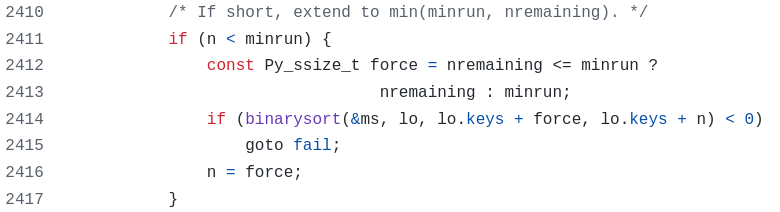
\includegraphics[width=\textwidth, height=0.5\textheight]{docs/images/force}
\end{center}
\end{figure}
\end{itemize}
\end{frame}